\comment{Results here, in past tense.}\\
To have a compact manner of referring to a specific implemented network structure, we introduce a new notation. A network with a specific architecture will hereby be referred to as \network{\textit{nodes by layer}}{\textit{groups by layer}}, where the superscript indicates the number of nodes in each hidden layer, chronologically, and the subscript indicates number of groups in each these layers. Whenever the number of groups equals the number of nodes, and we get an ordinary dense layer, we add a ReLU activation on the node output, and indicate it with an asterisk $*$. As an example, if a network has three layers: 32 nodes and two nodes per group; 64 nodes and four nodes per group; and 16 nodes and one node per group with ReLU, it will be denoted as \network{32, 64, 16}{16, 16, *}. 



\subsection{Visualising Sparse Pathways}
    After training the channel-out network \network{8,8,8}{4,2,4} on the MNIST dataset, we got a final test accuracy of 84.09\%. The activation pathways are visualised in \cref{res:fig:LWTA_architecture}.
    \begin{figure}
        \begin{subfigure}{\linewidth}
            \centering
            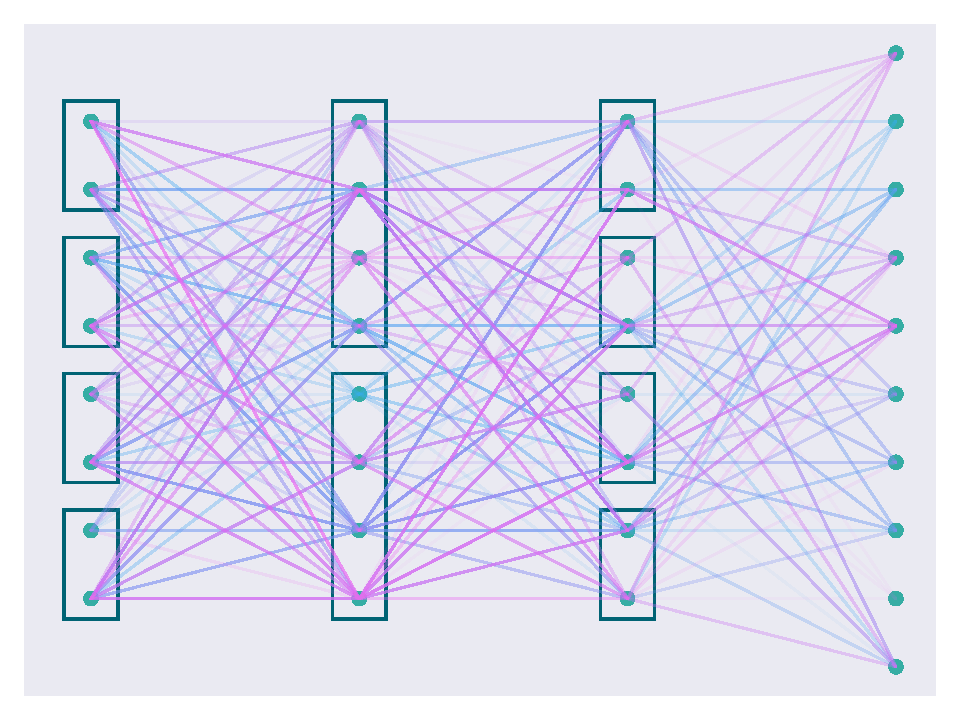
\includegraphics[width=\linewidth]{figs/LWTA_architecture_untrained.pdf}
            \caption{The untrained network predicting test images of zeros in blue and ones in pink.}
            \label[fig]{res:fig:LWTA_architecture_untrained}
        \end{subfigure}
        \begin{subfigure}{\linewidth}
            \centering
            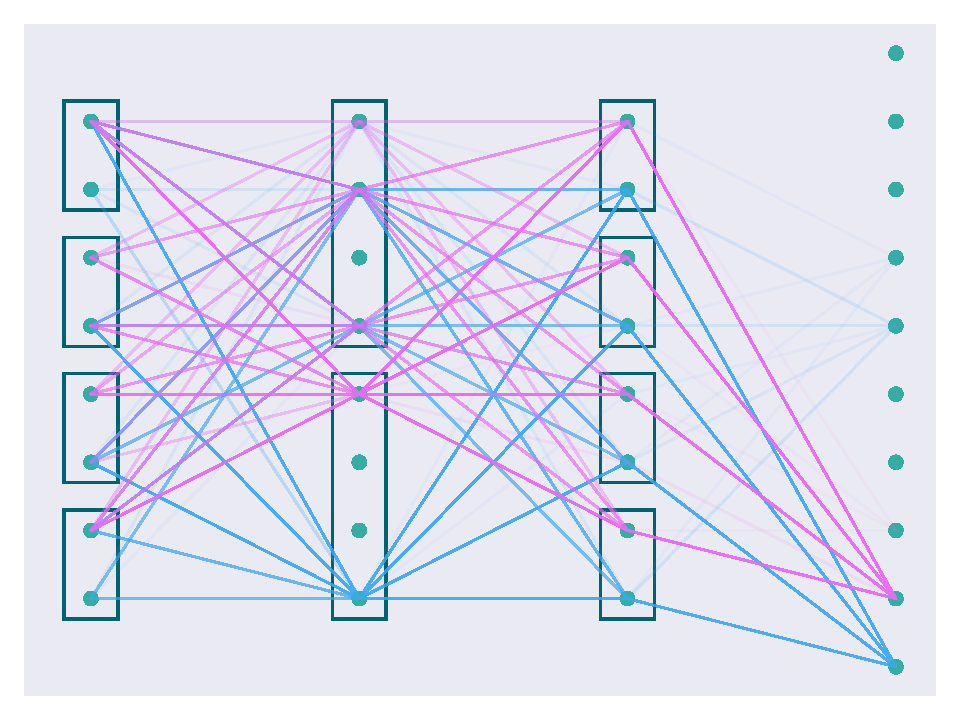
\includegraphics[width=\linewidth]{figs/LWTA_architecture_trained01.pdf}
            \caption{The trained network predicting test images of zeros in blue and ones in pink.}
            \label[fig]{res:fig:LWTA_architecture_trained01}
        \end{subfigure}
        \begin{subfigure}{\linewidth}
            \centering
            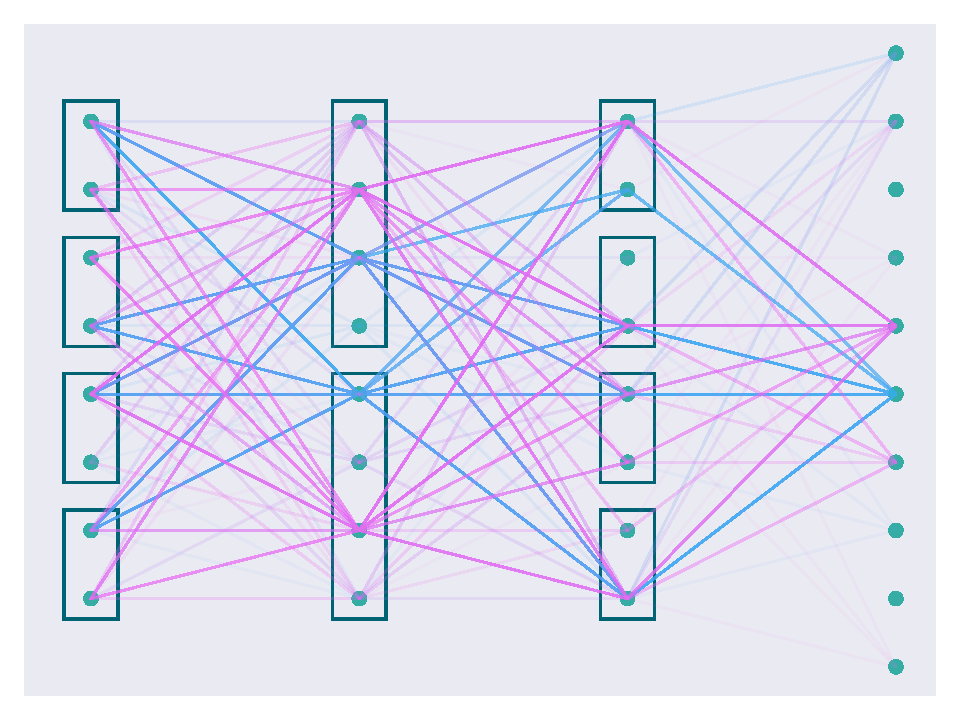
\includegraphics[width=\linewidth]{figs/LWTA_architecture_trained45.pdf}
            \caption{The trained network predicting test images of fours in blue and fives in pink.}
            \label[fig]{res:fig:LWTA_architecture_trained45}
        \end{subfigure}
        \caption{Illustrations of the active pathways as 100 input images from the MNIST test dataset belonging to two different classes are passed through a channel-out network. The network was trained on the full training dataset for 26 epochs before stopping early with $p=5$..}
        \label[fig]{res:fig:LWTA_architecture}
    \end{figure}

\subsection{Tuning LWTA Architecture}
    Tuning the architecture of our LWTA networks, we found the maxout network architecture \network{64,64}{32,16} with dropout to do the best on the CIFAR-10 dataset, achieving a test accuracy of 51.28\%. Likewise, the best performing channel-out network architecture was \network{64,16,64}{32,*,32} with L2 penalisation added, achieving a test accuracy of 50.69\%, slightly underperforming maxout. The ordinary ReLU dense network achieved an accuracy of 49.19\% on the test dataset with two layers of 32 nodes. The results are tabulated in \cref{res:tab:networks}.

    \renewcommand{\arraystretch}{2}
    \begin{table}[ht!]
        \centering
        \begin{tabular}{|l|c|c|c|}
        \hline
        & \textbf{Regularisation} & \textbf{Architecture} & \textbf{Accuracy} \\
        \hline
        \rowcolor{mint!20}
        \cellcolor{mint!20} & None & \network{64, 32, 64}{32, 16, 8} & 0.4909 \\ \cline{2-4} 
        \rowcolor{mint!20}
        \cellcolor{mint!20} & Ridge & \network{64, 32}{32, *}  & 0.5116 \\ \cline{2-4} 
        \rowcolor{mint!50}
        \cellcolor{mint!20} & Dropout & \network{64, 64}{32, 16} & 0.5128 \\ \cline{2-4} 
        \rowcolor{mint!20}
        \multirow{-4}{*}{\rotatebox[origin=c]{90}{Maxout}}{\cellcolor{mint!20}} & Both & \network{32, 64}{16, 16} & 0.4969 \\ \hline
        \rowcolor{maroon!20}
        \cellcolor{maroon!20} & None & \network{64, 16, 32}{16, 8, *} & 0.4823 \\ \cline{2-4} 
        \rowcolor{maroon!50}
        \cellcolor{maroon!20} & Ridge & \network{64, 16, 64}{32, *, 32} & 0.5069 \\ \cline{2-4} 
        \rowcolor{maroon!20}
        \cellcolor{maroon!20} & Dropout & \network{32, 16, 64}{16, *, 32} & 0.4790 \\ \cline{2-4} 
        \rowcolor{maroon!20}
        \multirow{-4}{*}{\rotatebox[origin=c]{90}{Channel-Out}}{\cellcolor{maroon!20}} & Both & \network{32, 64}{16, 32} & 0.4987 \\ \hline
        \rowcolor{cyan!20} 
        \cellcolor{cyan!20} & None & \network{32,32}{*,*} & 0.4843 \\ \cline{2-4} 
        \rowcolor{cyan!50} 
        \multirow{-2}{*}{\rotatebox[origin=c]{90}{Dense}}{\cellcolor{cyan!20} } & Ridge & \network{32,32}{*,*} & 0.4919 \\ \hline
        \end{tabular}
        \caption{Table of the best performing network architectures on the CIFAR-10 dataset. We used maxout, channel-out or dense ReLU layers and various combinations of dropout and ridge penalisation added.}
        \label[tab]{res:tab:networks}
    \end{table}
    \renewcommand{\arraystretch}{1}

    \begin{figure}
        \begin{subfigure}{\linewidth}
            \centering
            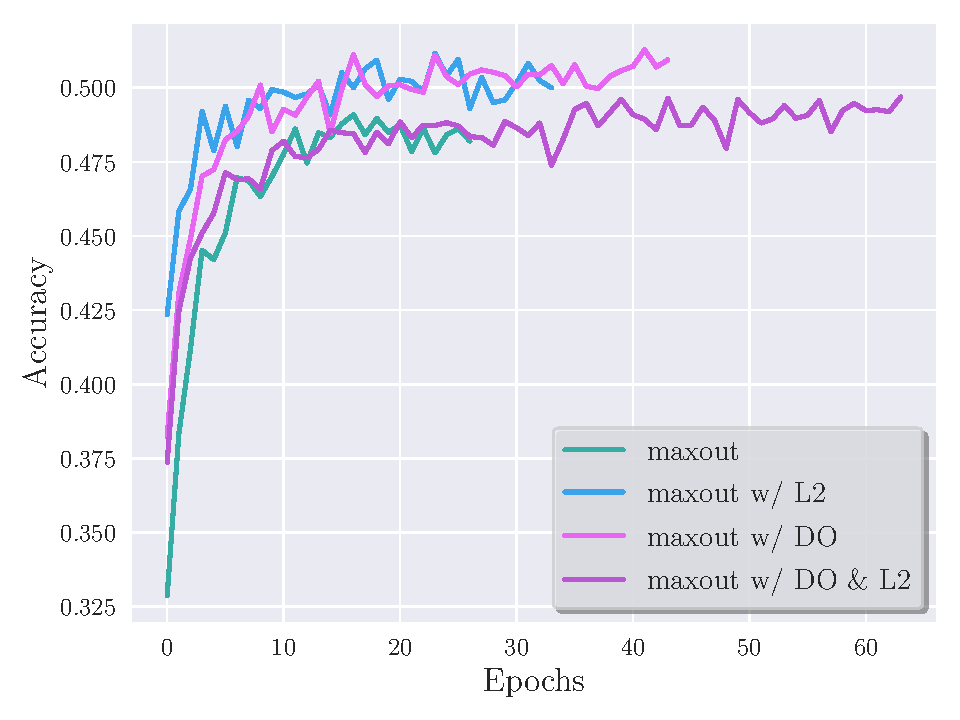
\includegraphics[width=\linewidth]{figs/best_models_maxout.pdf}
            \caption{The test accuracy history of the best performing maxout networks.}
            \label[fig]{res:fig:best_maxout}
        \end{subfigure}
        \begin{subfigure}{\linewidth}
            \centering
            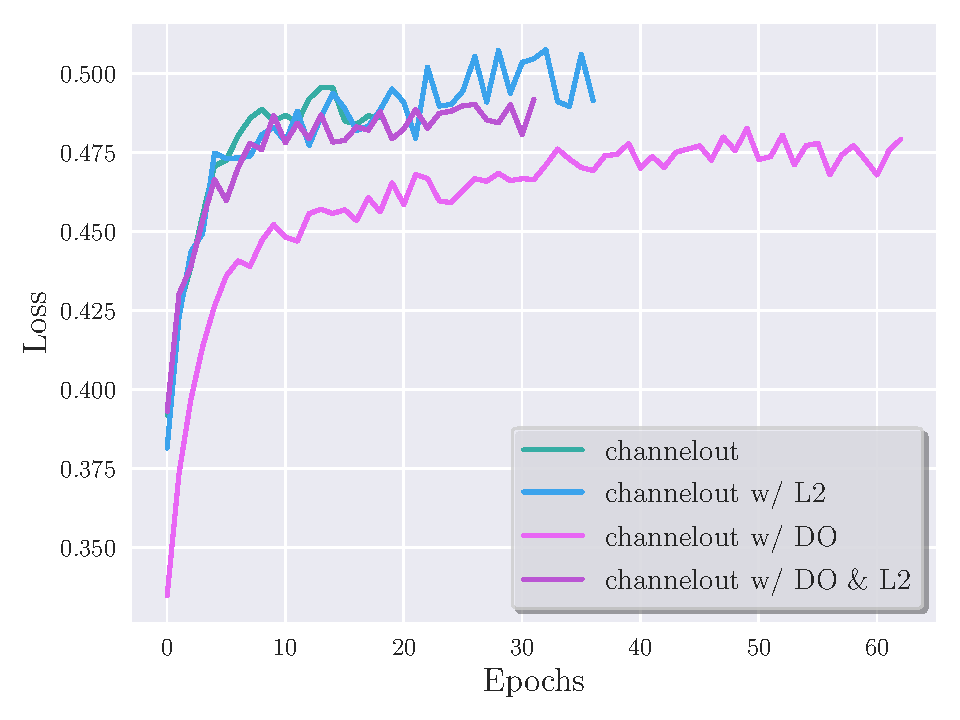
\includegraphics[width=\linewidth]{figs/best_models_channelout.pdf}
            \caption{The test accuracy history of the best performing channel-out networks.}
            \label[fig]{res:fig:best_channelout}
        \end{subfigure}
        \caption{The best performing LWTA models after tuning on the CIFAR-10 dataset were trained on the full training dataset and their test accuracy history is plotted here. For the network architecture of the various models see \cref{res:tab:networks}.}
        \label[fig]{res:fig:best_LWTA}
    \end{figure}
    \comment{Discussion note: Comment on the lack of resampling used here. -\Carl}

    \subsubsection{Premier League Dataset}
        \renewcommand{\arraystretch}{2}
        \begin{table}[ht!]
            \centering
            \begin{tabular}{|l|c|c|c|}
            \hline
            & \textbf{Regularisation} & \textbf{Architecture} & \textbf{Accuracy} \\
            \hline
            \rowcolor{mint!20}
            \cellcolor{mint!20} & None & \network{8,16}{*,8} & 0.5403 \\ \cline{2-4} 
            \rowcolor{mint!50}
            \multirow{-2}{*}{\rotatebox[origin=c]{90}{MO}}{\cellcolor{mint!20}} & Both & \network{16, 64}{8, 32} & 0.5806 \\ \hline
            \rowcolor{maroon!50}
            \cellcolor{maroon!20} & None & \network{8,64,16,64}{*,32,*,32} & 0.5484 \\ \cline{2-4} 
            \rowcolor{maroon!20}
            \multirow{-2}{*}{\rotatebox[origin=c]{90}{CO}}{\cellcolor{maroon!20}} & Both & \network{8, 64}{*, 32} & 0.4839 \\ \hline
            \rowcolor{cyan!20} 
            \cellcolor{cyan!20} & None & \network{16,16}{*,*} & 0.5161 \\ \cline{2-4} 
            \rowcolor{cyan!50} 
            \multirow{-2}{*}{\rotatebox[origin=c]{90}{Dense}}{\cellcolor{cyan!20} } & Ridge & \network{16,16}{*,*} & 0.5887 \\ \hline
            \end{tabular}
            \caption{Table of the best performing network architectures on the EPL dataset, with maxout, channel-out or dense ReLU layers and various combinations of dropout and ridge penalisation added.}
            \label[tab]{res:tab:EPL_networks}
        \end{table}
        \renewcommand{\arraystretch}{1}
    
        \begin{figure}
            \centering
            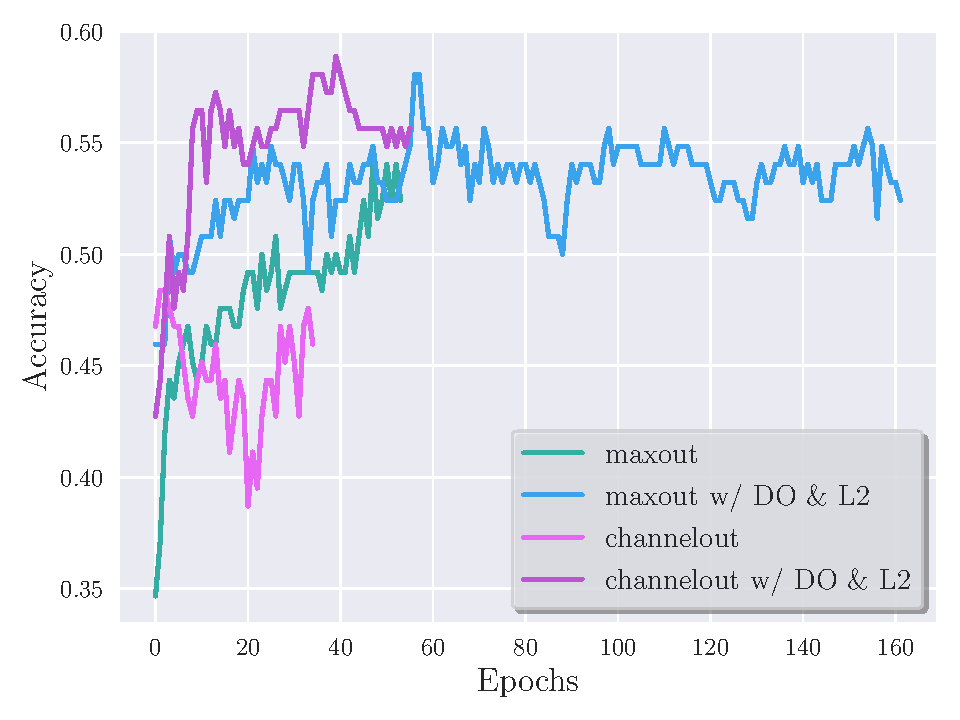
\includegraphics[width=\linewidth]{figs/best_models_EPL.pdf}
            \caption{The history accuracy on the test portion of the EPL dataset of the four best LWTA architectures, with and without regularisation methods added.}
            \label[fig]{res:fig:best_EPL}
        \end{figure}

\subsection{PCA on Premier League data}
    By performing PCA on the Premier League data we found its principal components. The explained variance as a function of principal components is plotted in figure~\ref{res:fig:explained_variance} as both a cumulative sum and histogram bars. As seen from the plot, 42 principal components explains 99 \% of the variance of the original features. Since this would reduce the dimensionality by approximately one half only, and we considered relatively few dimensions we decided not to use the principal components for further analysis. 
    \begin{figure}
        \centering
        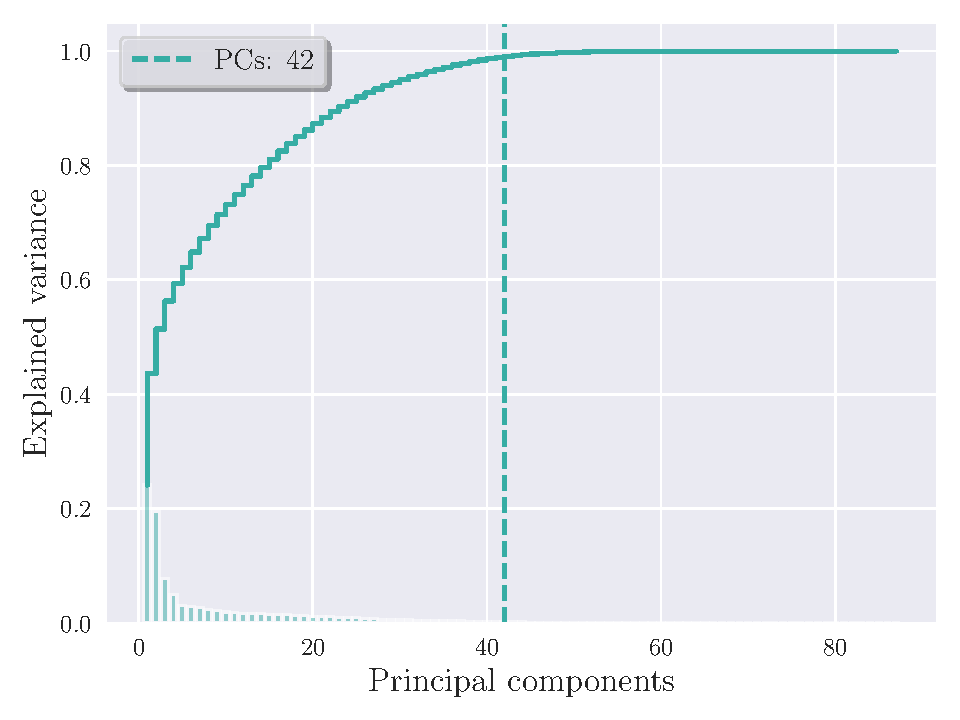
\includegraphics[width=\linewidth]{figs/pca_pl.pdf}
        \caption{Explained variance as function of the number of principal components, shown both as a cumulative step function and histogram bars showing the step increase for each component.}
        \label[fig]{res:fig:explained_variance}
    \end{figure}

